\documentclass[aspectratio=169]{beamer}
\setbeamertemplate{navigation symbols}{}
\usepackage{color, amsmath, comment, subfigure}
\usepackage{url}

\usepackage{hyperref}
\hypersetup{
    colorlinks=true,
    linkcolor=blue,
    filecolor=magenta,      
    urlcolor=cyan,
}

%%%%%%%%%%%%%%%%%%%%%%%%%%
\title[]{Pre-read for Tuesday, November 3:\\Disease modeling}
\author[]{Matthew J. Salganik}
\institute[]{}
\date[]{COS 597E/SOC 555 Limits to prediction\\Fall 2020, Princeton University}

\begin{document}
%%%%%%%%%%%%%%%%%%%%%%%%%%%
\frame{\titlepage}
%%%%%%%%%%%%%%%%%%%%%%%%%%%
\begin{frame}

\begin{center}
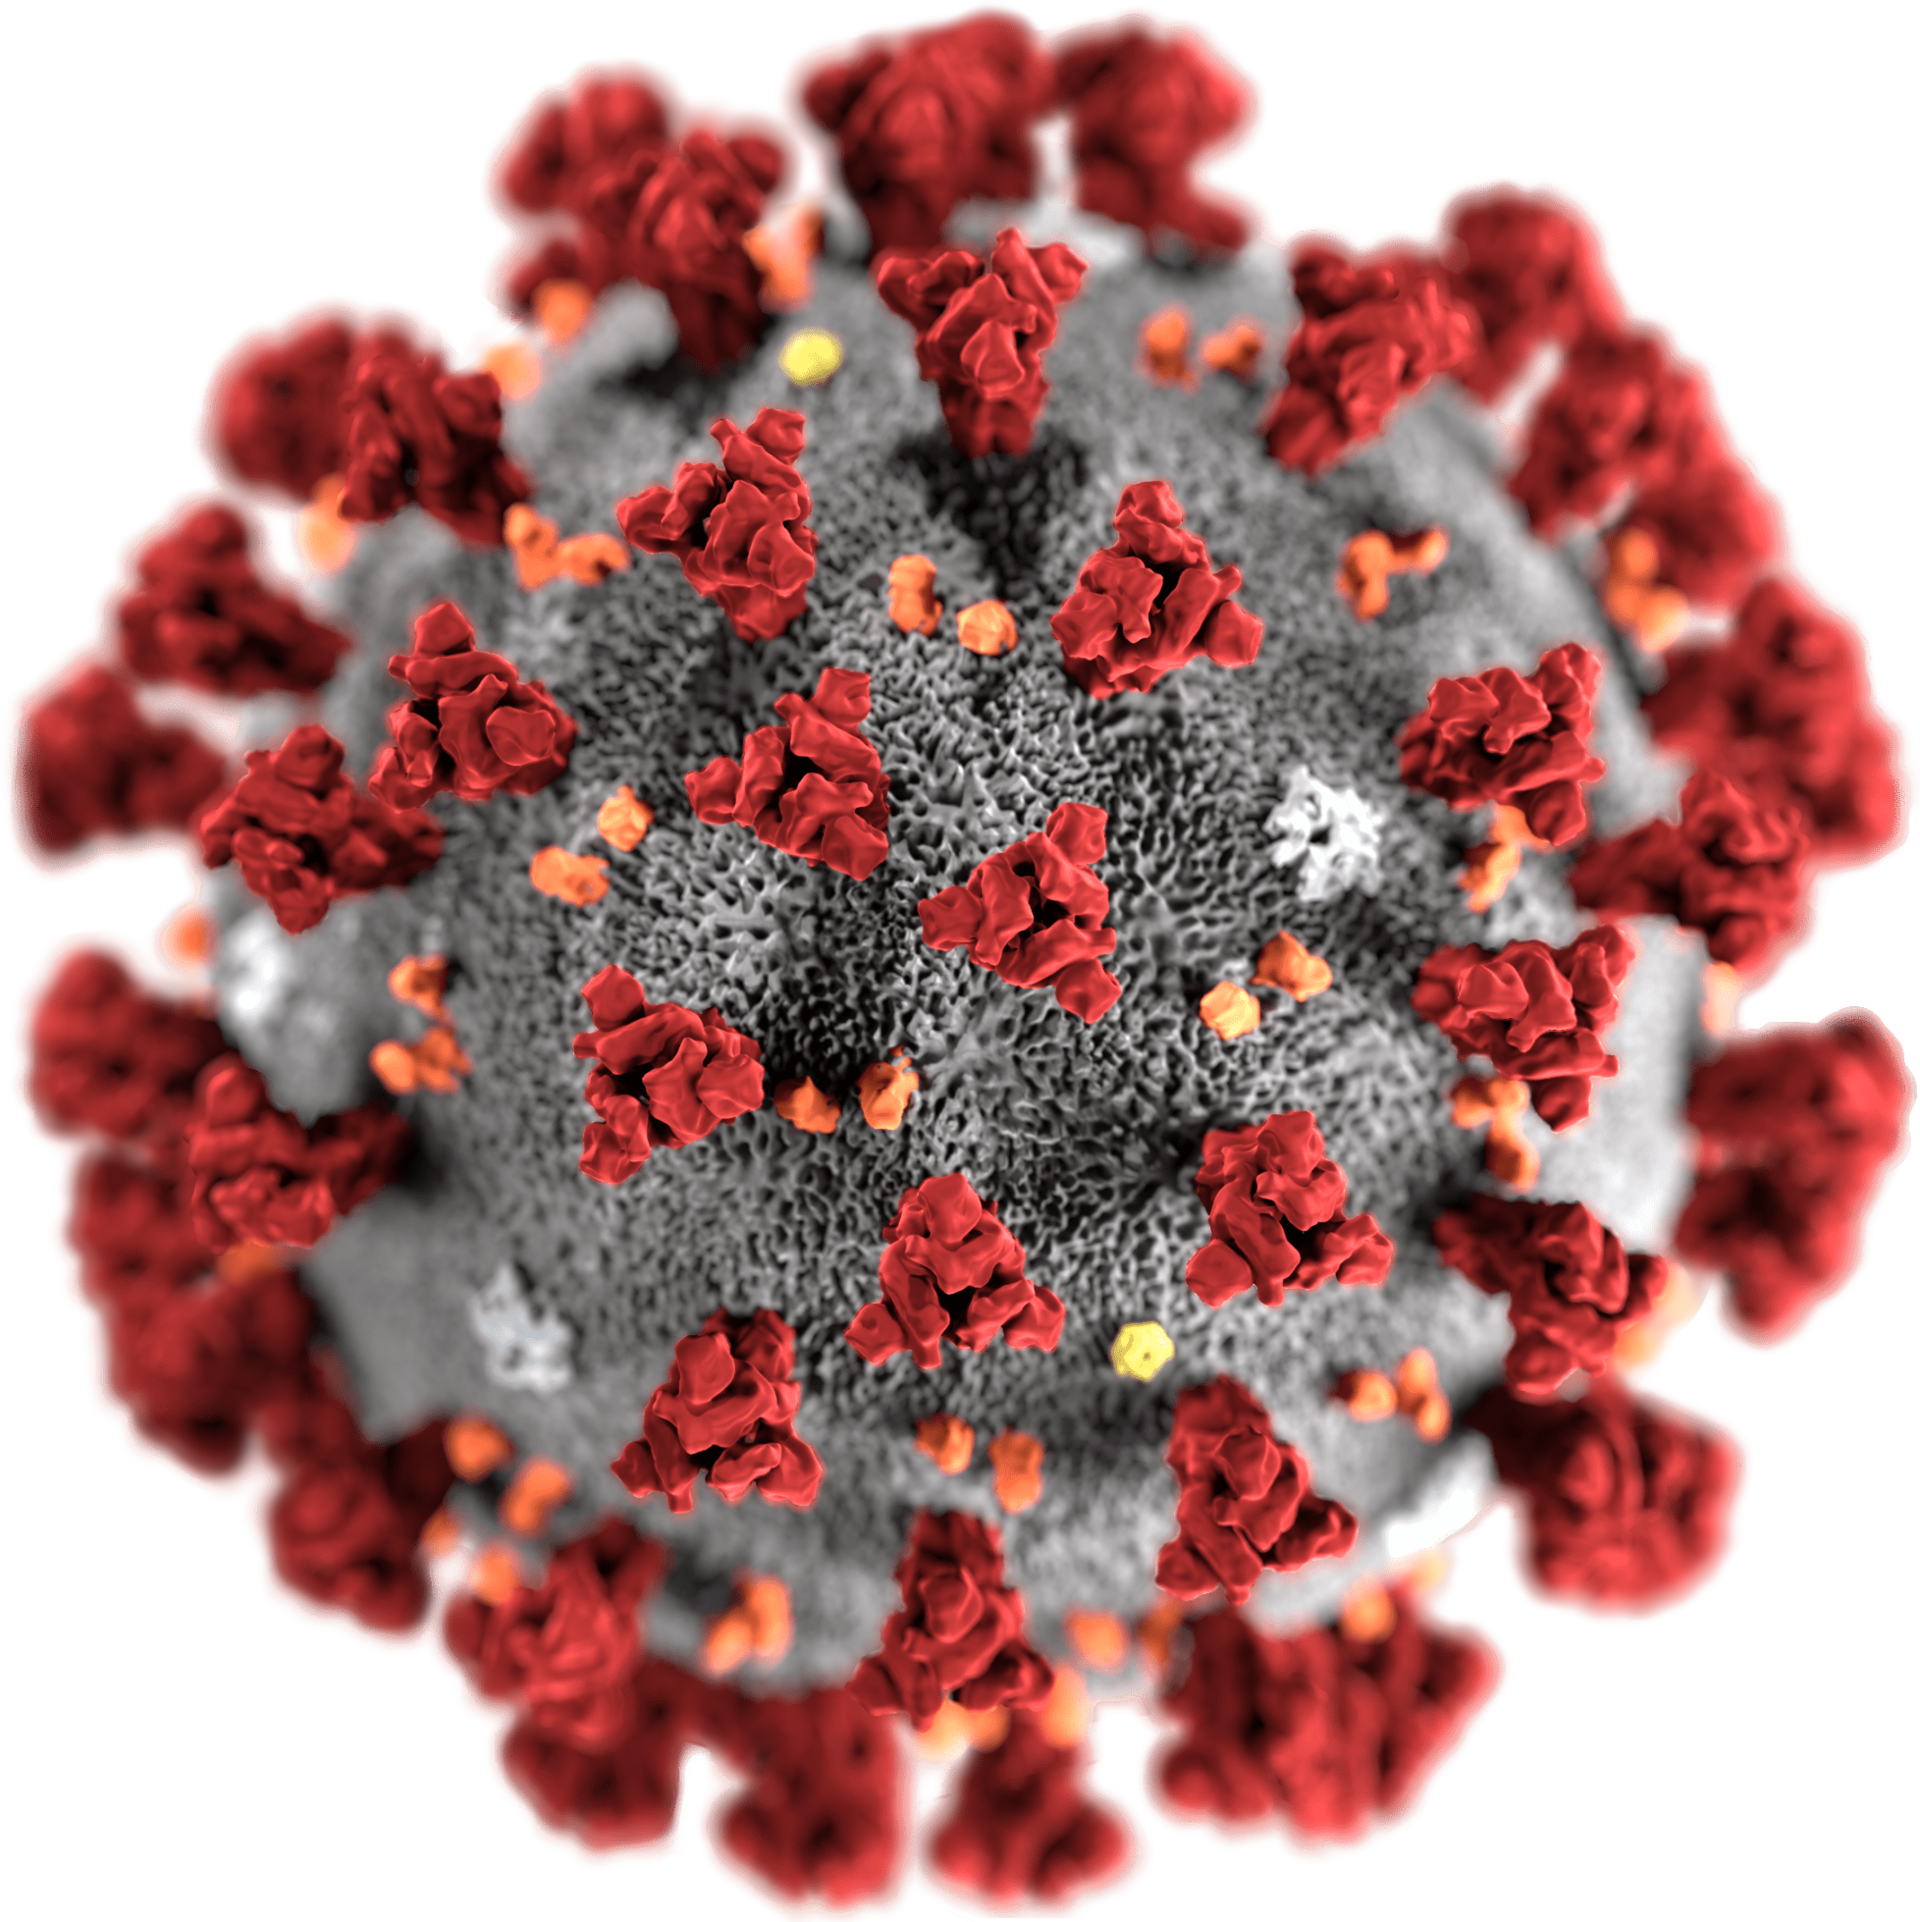
\includegraphics[height = 0.9\textheight]{figures/covid}
\end{center}

\vfill
\tiny{\url{https://phil.cdc.gov/Details.aspx?pid=23312}}
\end{frame}
%%%%%%%%%%%%%%%%%%%%%%%%%%%%%
\begin{frame}

\begin{center}
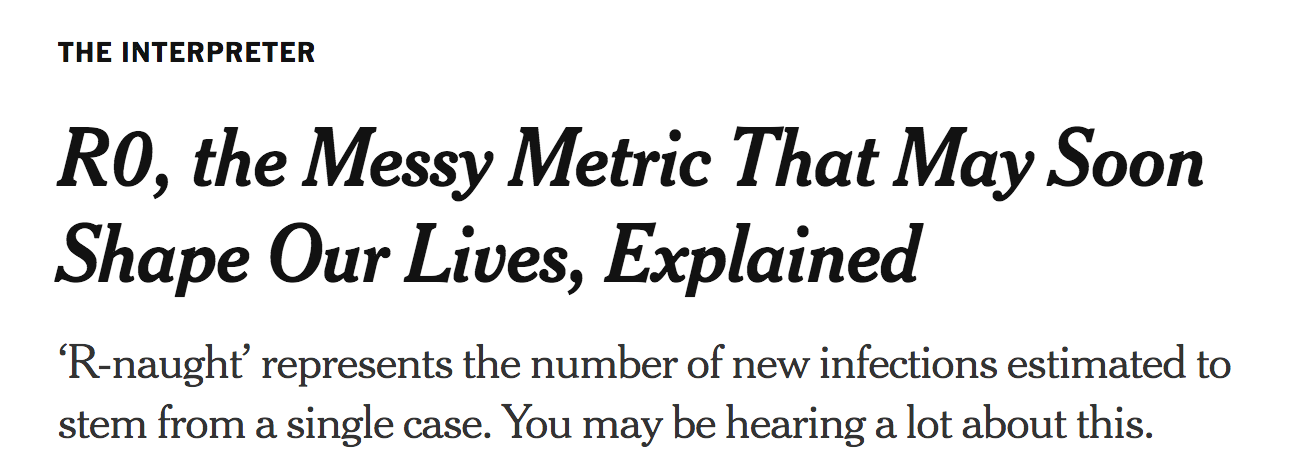
\includegraphics[width = 0.9\textwidth]{figures/fisher_r0_2020_title}
\end{center}

\end{frame}
%%%%%%%%%%%%%%%%%%%%%%%%%%%%
\begin{frame}

\begin{center}
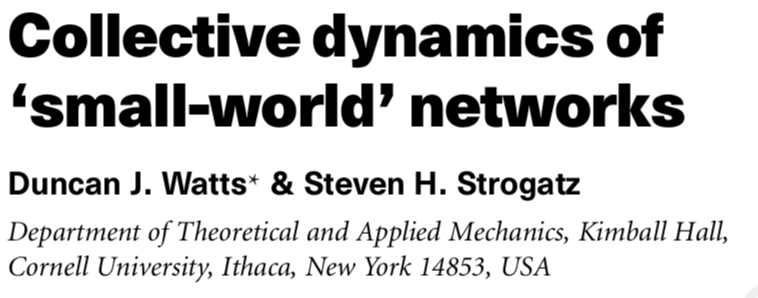
\includegraphics[width = 0.9\textwidth]{figures/watts_collective_1998_title}
\end{center}

\end{frame}
%%%%%%%%%%%%%%%%%%%%%%%%%%%%%
\begin{frame}

\begin{center}
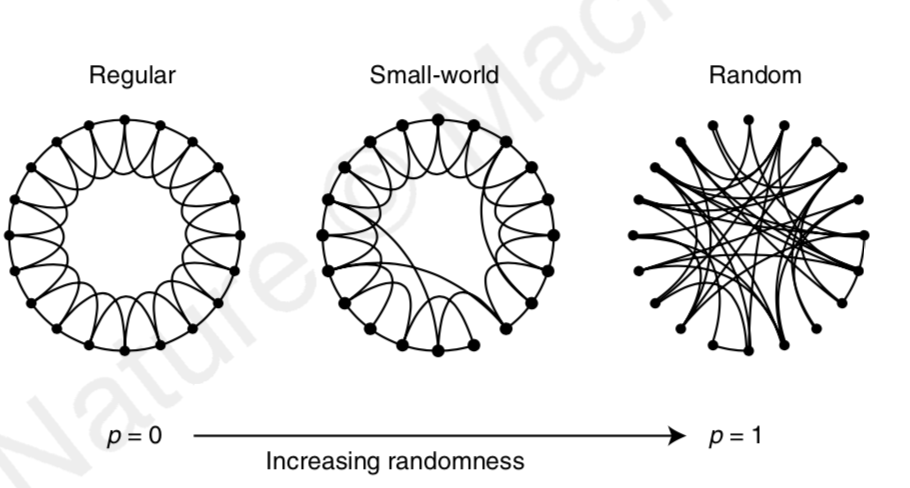
\includegraphics[width = 0.9\textwidth]{figures/watts_collective_1998_fig1}
\end{center}

\end{frame}
%%%%%%%%%%%%%%%%%%%%%%%%%%%%%
\begin{frame}

\begin{center}
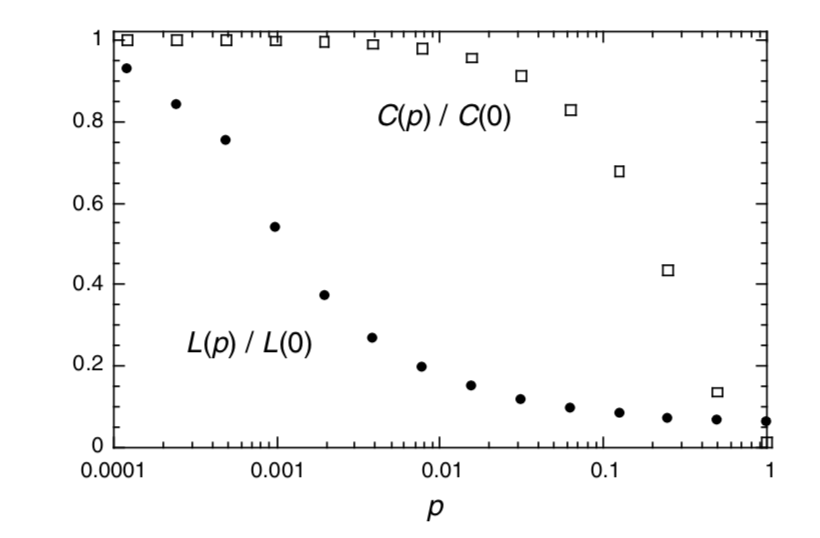
\includegraphics[width = 0.9\textwidth]{figures/watts_collective_1998_fig2}
\end{center}

\end{frame}
%%%%%%%%%%%%%%%%%%%%%%%%%%%%%
\begin{frame}

\begin{center}
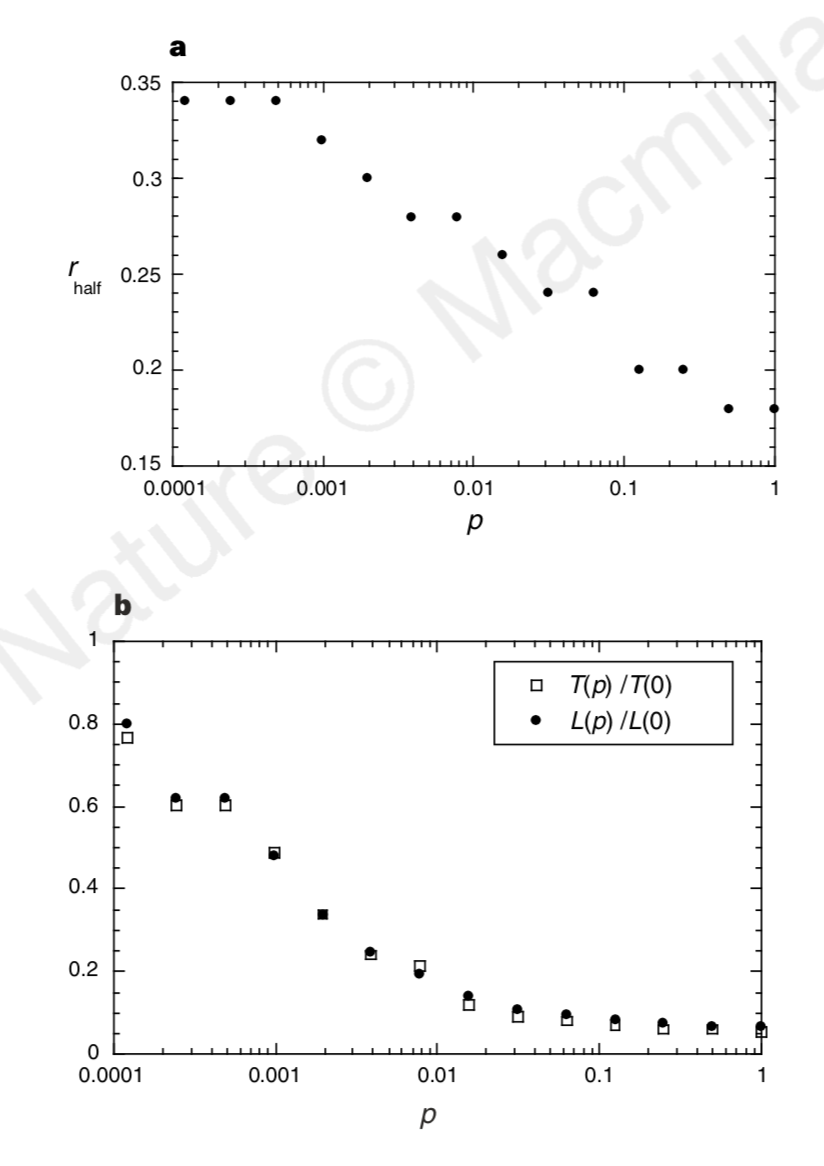
\includegraphics[height = 0.9\textheight]{figures/watts_collective_1998_fig3}
\end{center}

\end{frame}
%%%%%%%%%%%%%%%%%%%%%%%%%%%%%
\begin{frame}

Reading notes:
\begin{itemize}
\item What does it mean for predictability if the disease dynamics depend so sensitively on a single parameter that is hard to measure?  What if that sensitivity is only in a particular region of values?
\pause
\item This is a transformational paper in the study of networks so enjoy it
\end{itemize}

\end{frame}
%%%%%%%%%%%%%%%%%%%%%%%%%%%%%%
\begin{frame}

\begin{center}
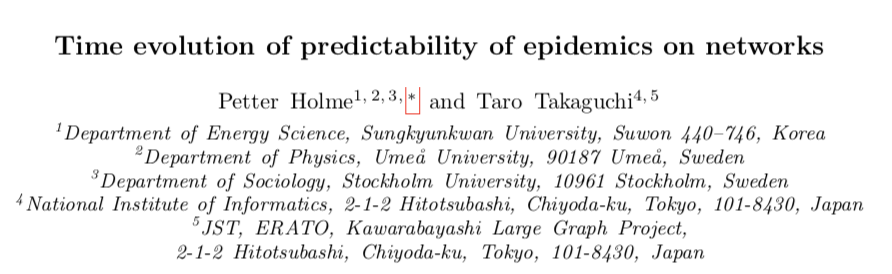
\includegraphics[width = 0.9\textwidth]{figures/holme_time_2015_title}
\end{center}

\end{frame}
%%%%%%%%%%%%%%%%%%%%%%%%%%%%%
\begin{frame}

\begin{center}
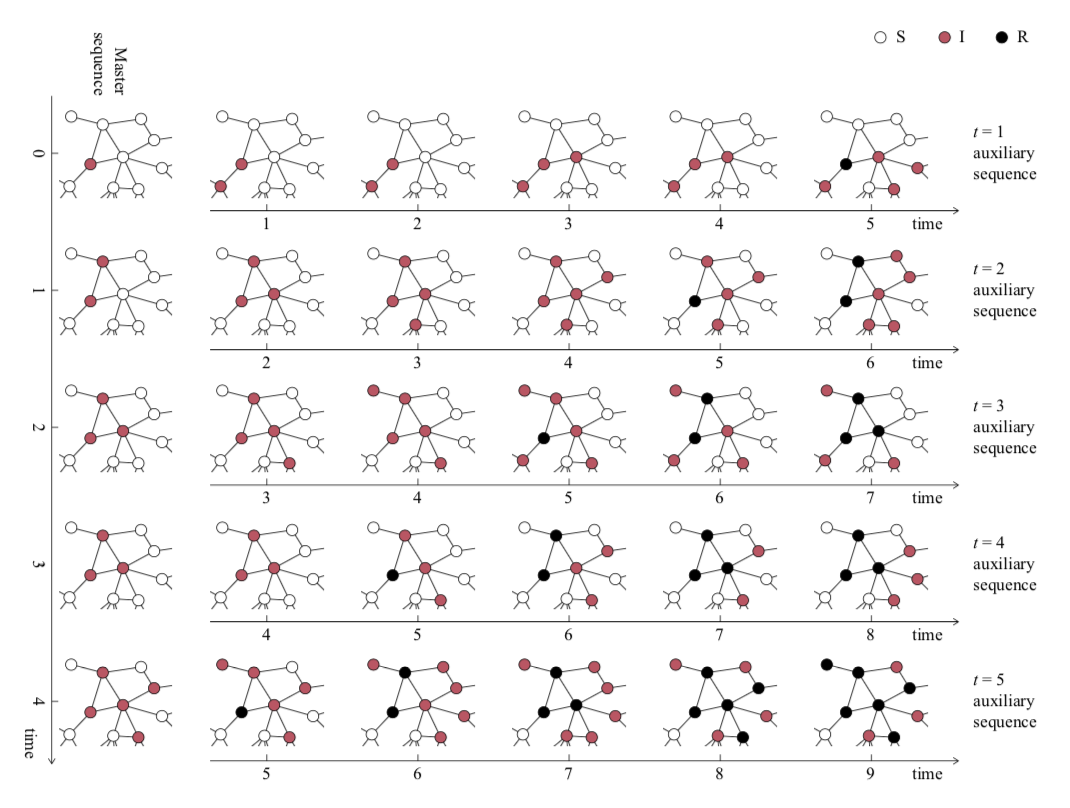
\includegraphics[height = 0.9\textheight]{figures/holme_time_2015_fig1}
\end{center}

\end{frame}
%%%%%%%%%%%%%%%%%%%%%%%%%%%%%
\begin{frame}

\begin{center}
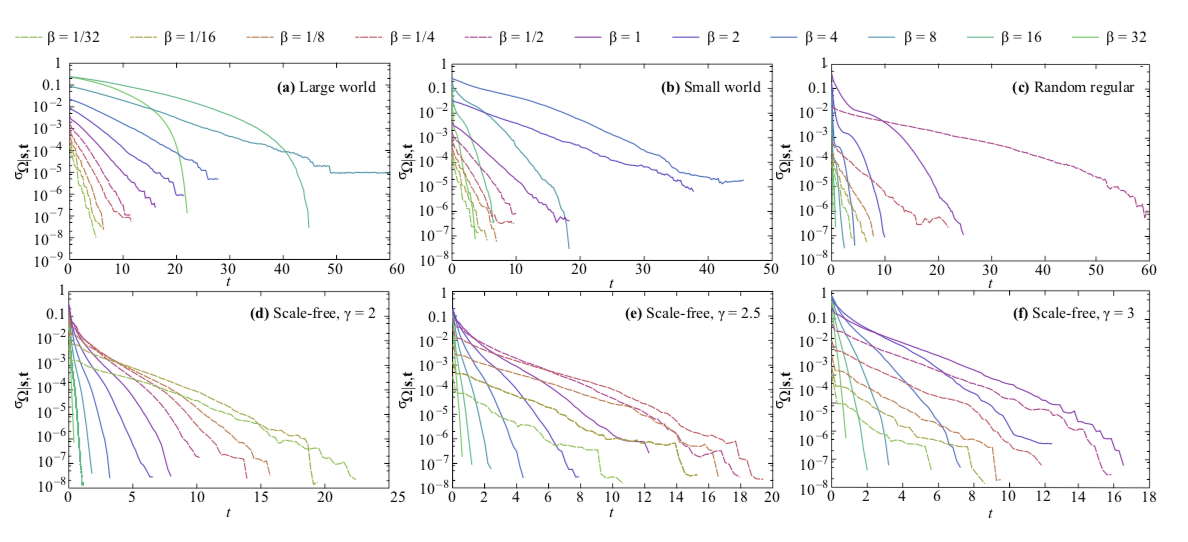
\includegraphics[width = 0.9\textwidth]{figures/holme_time_2015_fig3}
\end{center}

\end{frame}
%%%%%%%%%%%%%%%%%%%%%%%%%%%%%
\begin{frame}

Reading notes:
\begin{itemize}
\item If you are not familiar with it, pay attention to the SIR model 
\pause
\item Try to think about how this compares to other articles that we've read so far (e.g., Cheng et al's work on cascade prediction and the MusicLab experiments by Salganik et al)
\pause
\item Don't worry too much about the details of any specific claim. Focus on the big picture.
\end{itemize}

\end{frame}
%%%%%%%%%%%%%%%%%%%%%%%%%%%%%%
\begin{frame}

\begin{center}

\includegraphics[width = 0.9\textwidth]{figures/scarpino_on_2019_title}
\end{center}

\end{frame}
%%%%%%%%%%%%%%%%%%%%%%%%%%%%%%%
\begin{frame}

\begin{center}
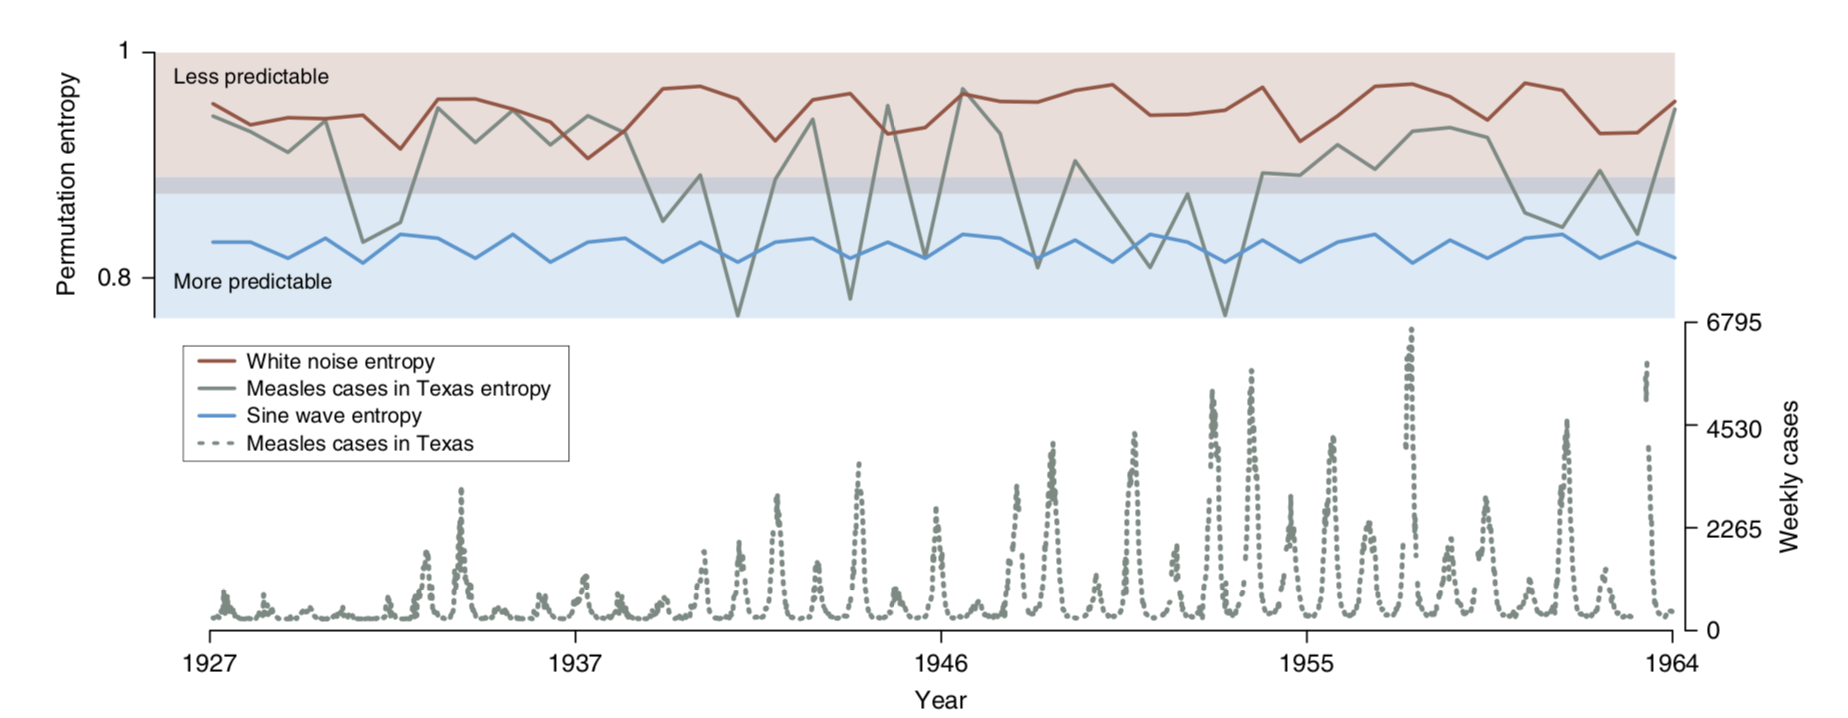
\includegraphics[width = 0.9\textwidth]{figures/scarpino_on_2019_fig1}
\end{center}

\end{frame}
%%%%%%%%%%%%%%%%%%%%%%%%%%%%%
\begin{frame}

\begin{center}
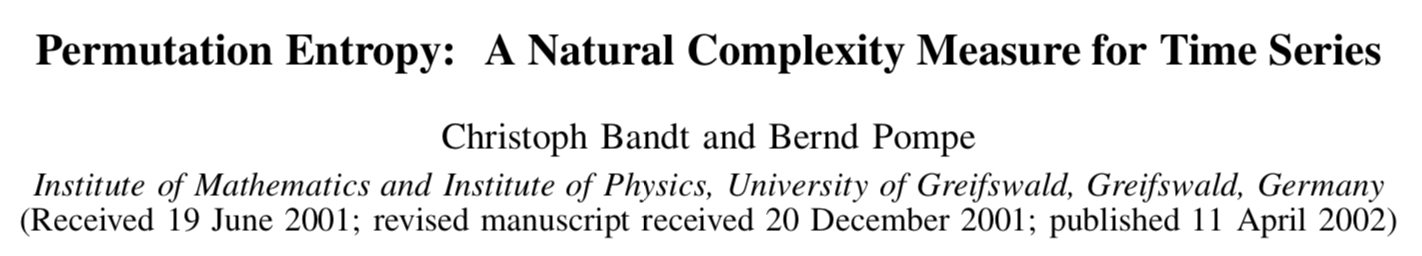
\includegraphics[width = 0.9\textwidth]{figures/bandt_permutation_2002_titie}
\end{center}

\end{frame}
%%%%%%%%%%%%%%%%%%%%%%%%%%%%%
\begin{frame}

\begin{center}
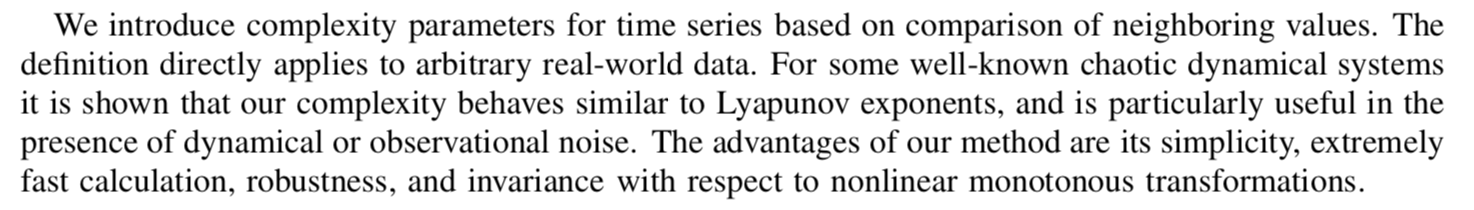
\includegraphics[width = 0.9\textwidth]{figures/bandt_permutation_2002_abstract}
\end{center}

\end{frame}
%%%%%%%%%%%%%%%%%%%%%%%%%%%%%
\begin{frame}

Example (from Bandt and Pompe, 2002):
$x = 4, 7, 9, 10, 6, 11, 3$

\begin{itemize}
\item 4 pairs for which $x_t < x_{t+1}$, represent these as \texttt{01}
\pause
\item 2 pairs for which $x_t > x_{t+1}$, represent these as \texttt{10}
\end{itemize}
\pause
Permutation entropy order $n = 2$ as a measure of the probabilities of the permutations \texttt{01} and \texttt{10}:

$H(2) = -(4/6) log_2(4/6) - (2/6) log_2(2/6) \approx 0.918$

\end{frame}
%%%%%%%%%%%%%%%%%%%%%%%%%%%%%
\begin{frame}

Example (from Bandt and Pompe, 2002):
$x = 4, 7, 9, 10, 6, 11, 3$

Next, we compare 3 consecutive values:
\begin{itemize}
\item (4, 7, 9) and (7, 9, 10) represent the permutation \texttt{012}
\item (9, 10, 6) and (6, 11, 3) correspond to the permutation \texttt{201} since $x_{t+2} <  x_{t} < x_{t+1}$ 
\item (10, 6, 11) has the permutation type \texttt{102}  since $x_{t+1} <  x_{t} < x_{t+2}$ 
\end{itemize}

The permutation entropy of order $n=3$:
$H(3) = -(2/5) log_2(2/5) - (2/5)log_2(2/5) - (1/5)log_2(1/5) \approx 1.512$

\end{frame}
%%%%%%%%%%%%%%%%%%%%%%%%%%%%%
\begin{frame}

\begin{center}
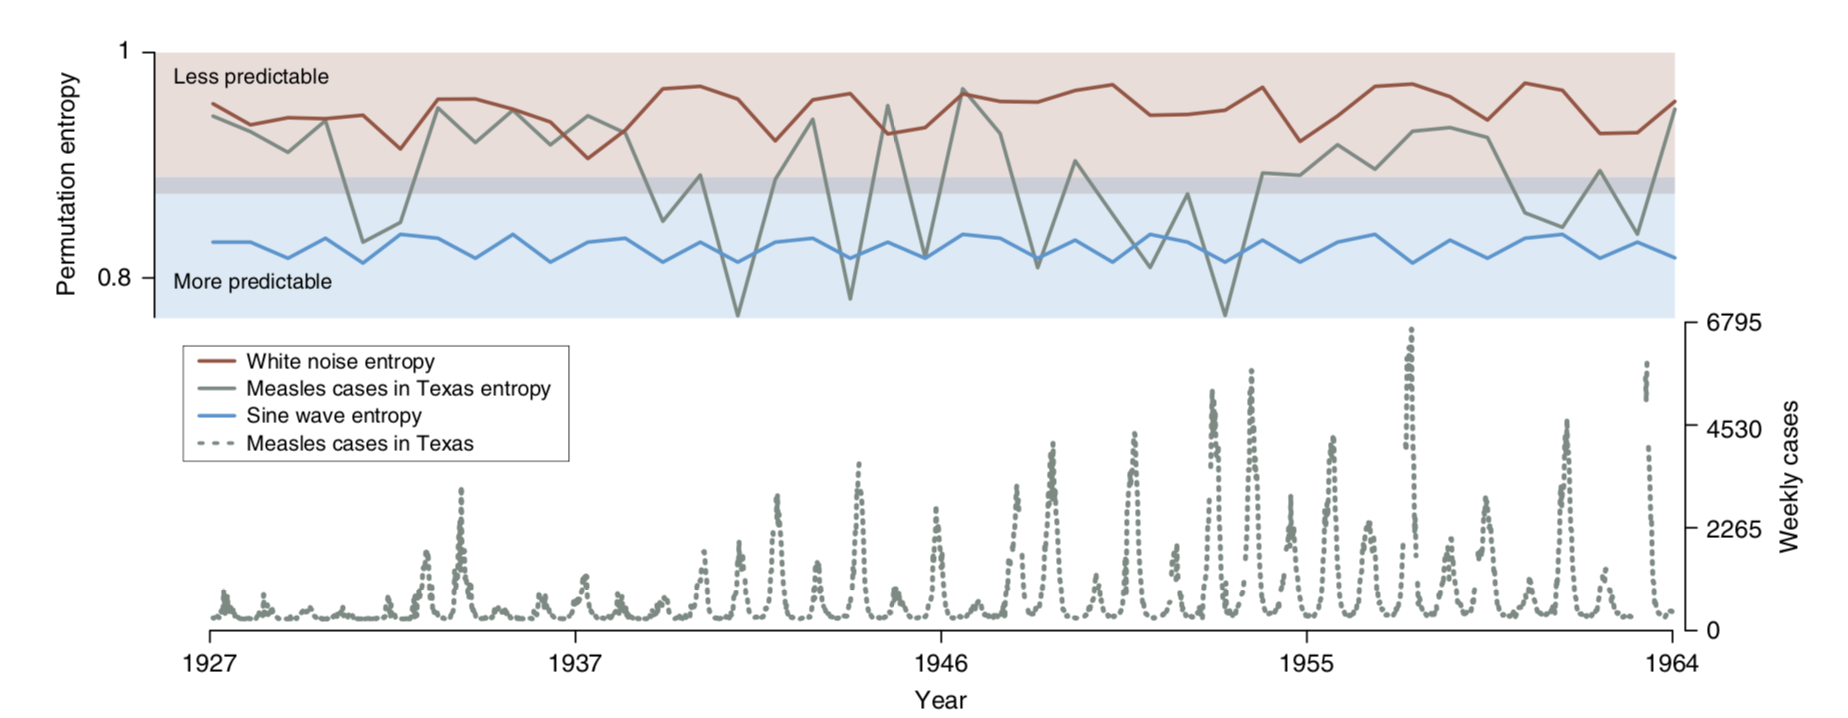
\includegraphics[width = 0.9\textwidth]{figures/scarpino_on_2019_fig1}
\end{center}

\end{frame}
%%%%%%%%%%%%%%%%%%%%%%%%%%%%%
\begin{frame}

\begin{center}
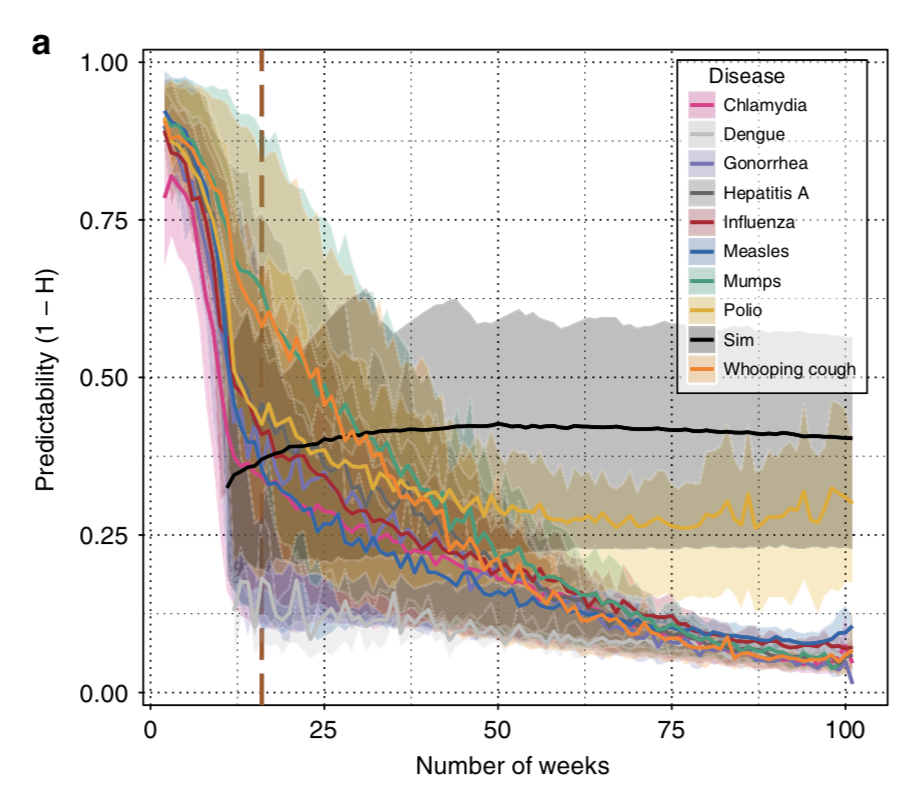
\includegraphics[width = 0.7\textwidth]{figures/scarpino_on_2019_fig2a}
\end{center}

\end{frame}
%%%%%%%%%%%%%%%%%%%%%%%%%%%%%
\begin{frame}

Reading notes:
\begin{itemize}
\item Do you think it is possible to learn something about the predictability of diseases this way?
\pause
\item Don't worry too much about the details of any specific claim. Focus on the big picture.
\end{itemize}

\end{frame}
%%%%%%%%%%%%%%%%%%%%%%%%%%%%%%
\begin{frame}

\begin{center}
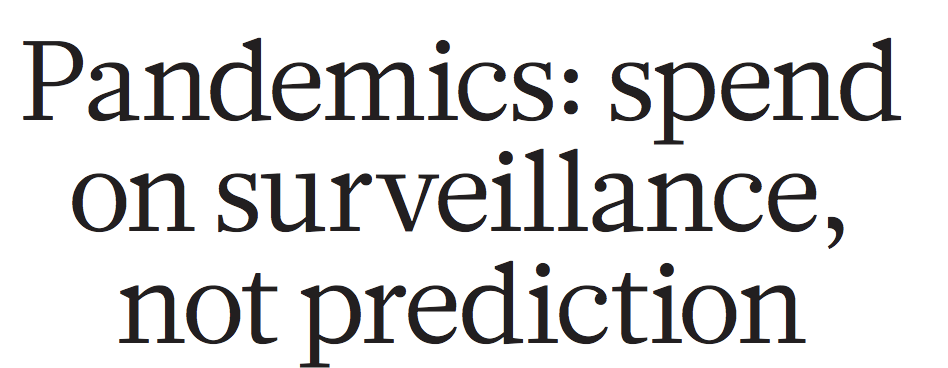
\includegraphics[width = 0.9\textwidth]{figures/holmes_pandemics_2018_title}
\end{center}

\end{frame}
%%%%%%%%%%%%%%%%%%%%%%%%%%%%%
\frame{\titlepage}


\end{document}
